\chapter{The Deliberate Press}
\label{ch:press}

\section{Four ways to press a button}

By 6~July the red button had been pressed four ways, in ascending order of intent: by
\emph{accident} (a held controller command parking the flange on it, ch.~\ref{ch:panel}); by
\emph{hand-published message} (a raw \texttt{JointState} to the bridge, ch.~\ref{ch:twin}); and
now by \emph{collision-aware plan} --- MoveIt given a model of the board, an operator-dragged
goal, and OMPL finding an arc \emph{around} the obstacle to a pre-press hover, followed by a
4\,cm approach that let PhysX compress the spring. The fourth way --- \emph{by code} --- is the
next chapter, and it is the one that goes to competition.

\begin{figure}[h]\centering
  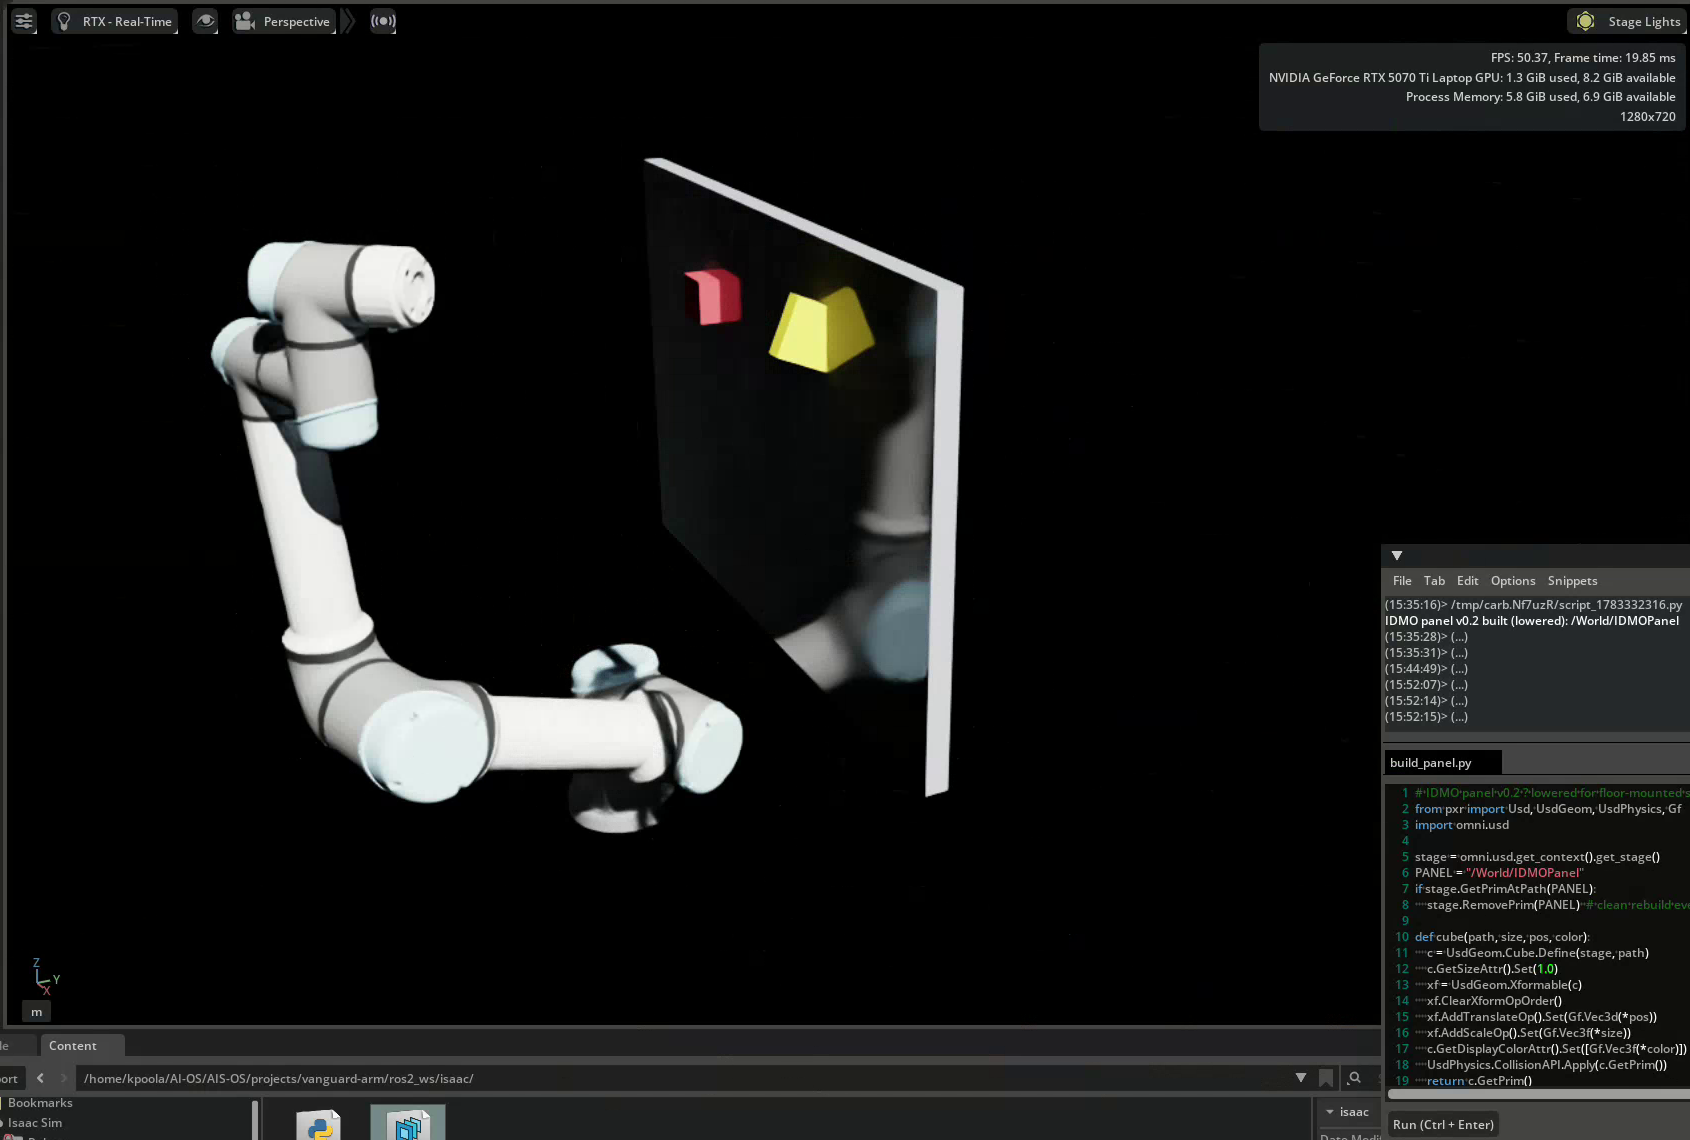
\includegraphics[width=0.9\linewidth]{figures/ch07_deliberate_press.png}
  \caption{Approach to the first deliberate press: MoveIt-planned, collision-checked path with
  the lowered panel (board at $z{=}0.72$, button and switch at $z{=}0.82$).}
\end{figure}

The planning-scene mechanics that made it work: MoveIt plans inside its \emph{own} world model,
populated by us --- one \texttt{PlanningScene} diff message adding a $0.62\times0.03\times0.42$
box (the board plus a 1\,cm skin). The button deliberately stays \emph{out} of the model so the
planner is allowed to touch it. RViz is where you aim; Isaac is where truth happens --- the
button exists only in the latter.

\section{Workspace analysis beats wishful dragging}

The first press attempt failed for a reason older than software: \textbf{reach}. The button at
$z{=}1.10$ sat ${\sim}1.03$\,m from the floor-mounted UR5e's shoulder --- beyond its 0.85\,m
envelope. The operator noticed before the math did (``the button might be too far up''). Fix:
lower the panel to $z{=}0.72/0.82$ --- moving the world, not straining the robot. The true
IRC height (panel up to 1.5\,m) returns in Phase~1, when the arm gains what the real rover
gives it: a deck-height pedestal. Recorded here so the pedestal doesn't get forgotten:
\emph{the stand-in's workspace is not the rover's workspace.}

\section{Mistakes log}

\begin{lesson}
\textbf{Restart order matters: consumers after providers.} After the controller stack was
killed and relaunched, MoveIt kept a dead handle to the \emph{old} controller: Plan produced a
cheerful purple ghost; Execute went nowhere. \texttt{move\_group} discovers controllers at
startup, so anything that \emph{uses} controllers must restart \emph{after} them. Clean
bring-up order, now doctrine: Isaac $\to$ control stack $\to$ MoveIt. Restart something
upstream, restart everything downstream.
\end{lesson}

\begin{lesson}
\textbf{Collision objects are double-edged.} When the panel (and its green box) moved down into
the parked arm, the start state itself became illegal --- \texttt{Failed} on every Plan, since
the planner validates both ends. The operator diagnosed it from the GUI alone (``the starting
state is lodged in the control panel'') --- exactly right. Escape: a \emph{raw} controller
command (the action interface checks nothing --- ch.~\ref{ch:controllers}'s missing guard,
repurposed as a rescue tool) folding the arm up and back. Habits adopted: retreat the arm
\emph{before} moving furniture; when Plan fails instantly, check the start state before blaming
the planner.
\end{lesson}

\begin{lesson}
\textbf{Two masters, one arm --- the container remembers.} The arm ``moved randomly'': a
controller manager from the \emph{previous day's session} was still alive inside the 3-day-old
container, and the fresh launch stacked a second one on top. Two JTCs holding different poses
wander the arm between them. \texttt{pgrep -fa ros2\_control\_node} before any launch;
``container up 3 days'' is a warning label, not a comfort.
\end{lesson}

\begin{lesson}
\textbf{Aim in the world model, verify in the simulator.} RViz shows only what MoveIt knows
(robot, TF, published boxes) --- no button, no switch. Operators aim at \emph{coordinates}
(12\,cm left of board center, 10\,cm up, 6\,cm off the face) with Isaac visible alongside for
ground truth. This split is permanent: the skill code will aim by coordinates too.
\end{lesson}

\section{Where this leaves us}

One full IDMO operation --- approach, contact, spring-back, retreat --- is now repeatable on
demand through the planner, with the button's own joint state as the scoring instrument
(${\sim}8$\,mm depressed, ${\sim}0$ released). Every piece of the press exists as something a
program can do: publish a scene, plan to a pose, approach, read a joint, retreat. Chapter 8
assembles exactly those calls into \texttt{press\_button} --- the first of the six skills.
